\newpage

\section{PLAN DE INVESTIGACIÓN}
    \subsection{Realidad problemática}
        Según cifras establecidas por grandes empresas del medio como Cisco,  se puede predecir que en un futuro próximo tendremos cerca de 50 a 100 mil millones de objetos conectados electrónicamente a internet, es un cifra bastante colosal que poco a poco genera problemas debido a las tecnologías que se usan actualmente para poder desplegar cualquier proyecto basado en Internet de las Cosas.\par
        Desde el año 2000 se viene hablando sobre Internet de las Cosas y cómo cimentar las bases exactas para lograr darle el mejor soporte en tecnologías de comunicación, pero de acuerdo a ciertos autores, cada solución que se plantean para un problema es momentánea, es decir, funciona bajo el paradigma de una enfermedad terminal, dónde cura la herida por un cierto tiempo pero si no se plantean nuevas formas mas sofisiticadas para solucionar el problema, volvemos a caer en el mismo hoyo. Tal es el caso de las redes 4G que han permitido que IoT no tenga problemas con la conectividad por mucho tiempo, pero la gran cantidad de dispositivos ha obligado a esta tecnología a evolucionar y lidiar con el problema que presenta IoT.\par
        La tecnología más usada por parte de IoT, es Cloud Computing, dicha tecnología es buena solución ya que nos provee alto poder de cómputo, pero ya que nos enfrentamos a un contexto en el cual tenemos que lidiar con grandes cantidades de datos provenientes de diferentes puntos de información, esta deja de ser una buena solución,  su arquitectura centralizada provoca grandes problemas, uno de ellos la latencia. Al enfrentarse a una masiva cantidad de datos, las 24 horas del dia, Cloud Computing no la pasa nada bien, su arquitectura centralizada hace que IoT no despliegue todo su potencial. \par
        Partiendo de esta problemática nace Fog Computing, una solución que viene de una u otra manera  a lidiar con la latencia que se presenta en la entrega de los datos, planteando un arquitectura distribuida y más local al lugar donde se generan los datos; además de eso Fog Computing lanza la idea de aprovechar la capacidad de cómputo de los dispositivos finales, pero es ahí donde tenemos un nuevo problema, los dispositivos finales cuentan con recursos limitados; recursos que son accesibles en cuestiones económicas debido al auge y el crecimiento de IoT pero con limitaciones en su nivel de procesamiento y almacenamiento.\par
        El escenario antes mencionado nos enfrenta al siguiente problema 
    \subsection{Antecedentes}
        \vskip 0.3cm
        {\bf\cite{alfuqaha2015}} expresan que IoT está habilitado por los últimos desarrollos en RFID, sensores inteligentes, tecnologías de comunicación y protocolos de Internet. Donde la premisa básica es que los sensores inteligentes colaboren directamente sin participación humana para ofrecer una nueva clase de aplicaciones. También enfatizan en que la revolución actual en las tecnologías de Internet, dispositivos móviles y máquina a máquina (M2M) se puede ver como la primera fase del IoT. En los próximos años,  esperan que IoT conecte diversas tecnologías para permitir nuevas aplicaciones conectando objetos físicos en apoyo de una toma de decisiones inteligente.\par
        Este paper nos muestra el panorama actual de IoT entorno a los ultimos avances tecnologicos de algunos campos y culmina enfatizando la necesidad de muchas aplicaciones con respecto a la evolucion de IoT.
        \vskip 0.3cm
        {\bf\cite{borgia2014}} habla sobre IoT como un nuevo paradigma que combina aspectos y tecnologías provenientes de diferentes enfoques. Donde la computación ubicua, el protocolo de Internet, las tecnologías de detección, las tecnologías de comunicación y los dispositivos integrados se fusionan para formar un sistema en el que el mundo real y digital se encuentran y están continuamente en interacción simbiótica. Además mencionan que la gran cantidad esperada de dispositivos interconectados y la gran cantidad de datos disponibles abren nuevas oportunidades para crear servicios que traerán beneficios tangibles a la sociedad, el medio ambiente, la economía y los ciudadanos individuales.\par
        Esta investigación nos aporta un enfoque donde la cantidad de dispositivos que serán conectados a internet en los proximos años, abre un sinfín de posibilidades entorno a la creacion de servicios en diferentes campos como la economía, el medio ambiente, etc.
        \vskip 0.3cm
        {\bf\cite{mahumd2018}} Esta investigación habla sobre IoT en el cuidado de la salud, y los problemas que existen relacionados a la latencia, carga de datos desigual y la heterogeneidad de las aplicaciones. Servicios de la computación en la nube han sido utilizados en este campo, sin embargo, la centralización geográfica de los centros de datos de la nube no ha podido solucionar del todo los problemas antes mencionados, por ello se habla de un interoperabilidad entre las arquitecturas Cloud y Fog Computing lo cual implica una compleja coordinación entre aplicaciones y servicios.\par
        Este paper nos brinda resultados esperados en cuanto a lo solución de dichos problemas, simulando el uso de la arquitectura Fog Computing con el software iFogSim.\par
        \vskip 0.3cm
        {\bf\cite{verma2015}} nos mencionan los problemas que presenta Cloud Computing como por ejemplo: limitación con respecto al equilibrio de la carga de datos y el alojamiento de centros de datos, los cuales crean un nivel de latencia de red grande e impredecible. Además, presentan como solución para dichos problemas a un nuevo modelo de computación llamado Fog Computing, el cual es análoga a la nube, con la única diferencia es que se encuentra en el borde de la red; otra ventaja es que las aplicaciones que requieren dependencia de ubicación pueden ser viables a través de ella. Y para finalizar, proponen una nueva arquitectura basada en el algoritmo de equilibrio de carga en el entorno de Fog Computing de manera menos compleja y efectiva, debido a la gran cantidad de usuarios finales los cuales aumentan cada día a un ritmo muy rápido. \par
        Y para culminar, dicha investigación nos brindá información acerca del gran poder que tiene Fog Computing frente a temas de latencia y su manera eficiente de como solucionarlo, además nos muestran un panorama donde la combinación entre Fog Computing y el algoritmo de equilibrio de carga logran ser un dupla perfecta frente a estos problemas.\par
        \vskip 0.3cm
        Con el transcurso de los años los dispositivos IoT requieren mayor espacio para poder almacenar datos, los cuales aumentan masivamente {\bf\citep{murazzo2017}}, habla de la necesidad de mejorar los tiempos de respuesta y la escalabilidad de sistemas; menciona ejemplos de aplicaciones web con datos masivos que podrían manejarse con técnicas de computación de alto rendimiento permitiendo que la velocidad de procesamiento mejore.\par
        Este paper nos indica los campos necesarios a investigar para lidiar con grandes volúmenes de datos, tales como: arquitecturas híbridas, problemas de datos masivos y las herramientas existentes para resolverlos, entre otros.\par
        \vskip 0.3cm
        {\bf\cite{mugen2015}}presentan una red de acceso de radio basado en Fog Computing (F-RAN) como propuesta para lograr alcanzar los objetivos propuestos para el sistema de comunicación inalámbrica de quinta generación (5G), los cuales son: alcanzar un crecimiento de la capacidad del sistema de al menos 1000 y el crecimiento de la eficiencia energética (EE) en un factor de al menos 10.   Además, resaltan que en las actuales redes propuestas los operadores necesitan desplegar una gran cantidad de RRH y HPN (Nodos de Alta Potencia) fijos en H-CRANs para cumplir con los requisitos de capacidad máxima, lo que los convierte en un serio desperdicio cuando el volumen de tráfico de entrega no es lo suficientemente grande. Por ende, proponen a Fog Computing como una buena alternativa frente a Cloud Computing, cuya propuesta viene a colocar una cantidad sustancial de almacenamiento, comunicación, control, configuración, medición y administración en el borde de una red, donde el procesamiento de señal de radio de colaboración (CRSP) no solo se puede ejecutar en un grupo de BBU centralizado en H-CRANs, sino que también se puede alojar en RRH e incluso en UEs "inteligentes" utilizables.\par
        Este trabajo nos aporta una aplicación importante de Fog Computing en un campo como las redes 5G, donde se busca lograr el aprovechamiento de los dispositivos finales (RRH) frente a las limitaciones que presenta la propuesta planteada con el fin de lograr los objetivos de 5G.\par     
        \begin{figure}[ht]
            \begin{center}
                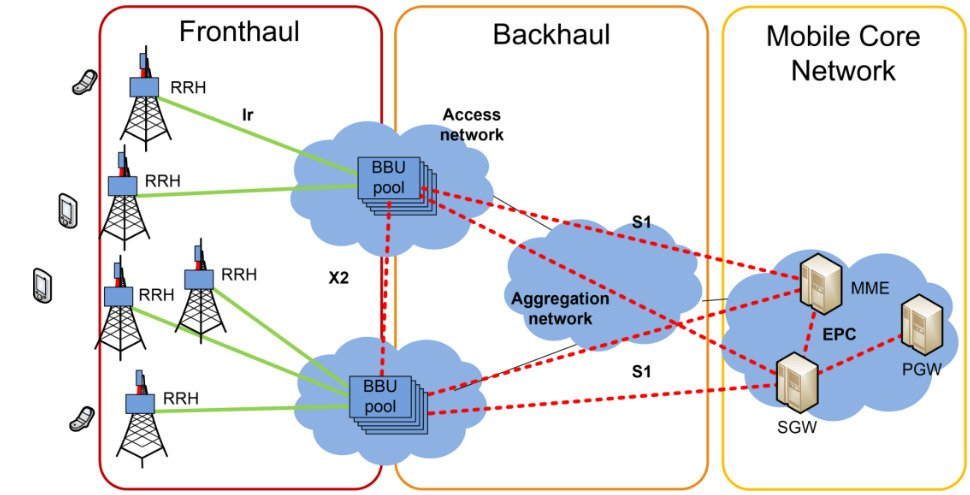
\includegraphics[width=.8\textwidth]{redFronthaul}
            \end{center}
        \end{figure}
        \begin{center}
            { Figura 1: Red de transporte Fronthaul - enlace entre RRH y BBU }\par 
            { Fuente: Aleksandra Checko (2015). }
        \end{center}   
        \vskip 0.3cm
        {\bf\cite{piccialli2018}} nos hablan de la cantidad de almacenamiento que se va generando por el incremento de dispositivos conectados a internet, en su mayoría debido a dispositivos IoT, y la estimada para el 2020; a su vez indica que el procesamiento actual de los datos no es ideal pero mejoraría con la inclusión de técnicas de computación paralela y distribuida.\par
        Como aporte, esta investigación reafirma nuestra idea de que al utilizar algoritmos paralelos podemos lograr una mejora notable en cuanto a la velocidad del procesamiento de los datos y por ende disminuir la latencia. \par
        \vskip 0.3cm
        {\bf\cite{shanmugapriya2018}} nos muestra un panorama donde una variante de un algoritmo de agrupamiento más reciente basado en el hallazgo rápido y la búsqueda de picos de densidad (CFS), tiene la capacidad de afrontar la agrupación de grandes cantidades de datos dinámicos en el Internet de las cosas industriales, donde muestra que dicha variación puede encontrar grupos de forma arbitraria y determinar la cantidad de clústeres automáticamente, solucionado de cierta manera las limitaciones que presentaba el algoritmo inicial frente al agrupamiento de grandes volúmenes de datos.\par
        Como aporte, esta investigación nos permite ver el potencial oculto que tiene este algoritmo CFS propuesto por Alessandro Laio, Alex Rodriguez y Maria d’Errico frente al agrupamiento de datos, que si bien es cierto tiene una limitación bien marcada frente al volumen de estos, podemos mejorarlo de acuerdo a nuestras necesidades o al problema que queremos resolver y obtener mejores resultados.\par

    \subsection{Justificación}
        \subsubsection{Justificación Informática}
            La necesidad de hacer frente a la problemática que vive actualmente la tecnología IoT y la que vivirá en los próximos años, nos hace pensar rápido en la manera de cómo mitigar esto y lograr solucionar los posible cuellos de botella que sufre y sufrirá esta tecnología si sigue tal y como esta. Por ende, la propuesta que planteamos nos hace involucrarnos a fondo en el paradigma donde cada objeto puede estar conectado a internet o de forma resumida, el Internet de las Cosas, también nos llama a sumergirnos en las diferentes arquitecturas enfocadas a dar soporte a esta tecnología y a lograr sacar a relucir todo el potencial de la computación paralela por medio de la creación de algoritmos de este tipo, que para procesar grandes cantidades de datos son mucho más eficaces que los comúnmente usados (algoritmos secuenciales), de tal manera que la complementación de estos nos permite plantear una nueva forma o enfoque de cómo solucionar la latencia que presenta IoT frente a un contexto donde se generar una gran cantidad de información de manera distribuida y la enorme necesidad de analizar toda esta data.
        \subsubsection{Justificación Organizacional}
            Frente al gran crecimiento de la cantidad de dispositivos conectados a internet y el problema de conectividad que enfrenta actualmente la tecnología IoT, encontramos un terreno donde el tema de la entrega de datos puede sufrir grandes complicaciones debido a factores como: la centralización que presenta la arquitectura sobre la cual funciona la mayoría de proyectos IoT y la gigantesca información proveniente de dispositivos finales que se necesitan procesar; conociendo este complicado panorama es que se necesita tener una solución frente al tema de la latencia existente en la transmisión de datos, por lo cual proponemos desarrollar un mecanismo concebido gracias a la complementación entre la arquitectura Fog Computing y algoritmos paralelos, permitiendo lograr reducir los tiempos de transmisión de datos entre los dispositivos donde se originan de los datos y los servidores alojados en la nube o centros de datos. De esta manera, se busca lograr que cada idea o proyecto sobre IoT, principalmente aquellos que manejan grandes cantidades de información de diferentes puntos de origen, no tengan complicaciones con respecto al tiempo de la transmisión de datos y el tema de análisis de la información se desarrolle la mejor manera posible.
    \subsection{Problema}
        ¿De qué manera se podría reducir la elevada latencia generada por las constantes peticiones desde los dispositivos IoT al servidor?\par
    \subsection{Hipótesis}
        Utilizando Fog Computing como arquitectura distribuida para poder descentralizar las cargas que presentaba IoT con Cloud Computing e implementando algoritmos paralelos en cada punto donde se procesa la información se podrá reducir la latencia de las peticiones al servidor.\par
    \subsection{Variables}
        \subsubsection{Variable Independiente}
            \begin{table}[h!]
                \centering
                \begin{tabular}{|p{3cm}|p{3cm}|p{3cm}|p{3cm}|} \hline
                    
                %%%%%%%    CABECERA      %%%%%%%    
                
                \textit{{\bf{Variable}}} &
                \textit{{\bf{Definición Conceptual}}} &
                \textit{{\bf{Dimensiones}}} &
                \textit{{\bf{Indicadores}}}
                \\ \hline

                %%%%%%%%    FILA 1   %%%%%%%
                % COLUMNA 1 %
                Algoritmos paralelos sobre la arquitectura Fog Computing &
                % COLUMNA 2 %
                Algoritmos enfocados al uso de varios procesadores trabajando juntos para resolver una tarea común &
                % COLUMNA 3 %
                Rendimiento de los Algoritmos Paralelos &
                % COLUMNA 4 %
                Tiempo de ejecución \par
                Aceleración (speedup) 
                \begin{equation*}\label{}
                    SU = \frac{Ts}{Tp}
                \end{equation*}   
                Eficiencia (efficiency) 
                \begin{equation*}\label{}
                    E(n) = \frac{S(n)}{n}
                \end{equation*}                

                \\ \hline

                \end{tabular}
            \end{table}
        \subsubsection{Variable Dependiente}
            \begin{table}[h!]
                \centering
                \begin{tabular}{|p{3cm}|p{3cm}|p{3cm}|p{3cm}|} \hline
                    
                %%%%%%%    CABECERA      %%%%%%%    
                
                \textit{{\bf{Variable}}} &
                \textit{{\bf{Definición Conceptual}}} &
                \textit{{\bf{Dimensiones}}} &
                \textit{{\bf{Indicadores}}}
                \\ \hline

                %%%%%%%%    FILA 1   %%%%%%%
                % COLUMNA 1 %
                Latencia en el Internet de las Cosas &
                % COLUMNA 2 %
                Retardo existente en la entrega de datos dentro la red &
                % COLUMNA 3 %
                Latencia &
                % COLUMNA 4 %
                Tiempo existente entre la transmisión y la recepción de los datos. 
                \\ \hline

                \end{tabular}
            \end{table}
    \subsection{Objetivos}
        \subsubsection{Objetivo general}
            Disminuir el tiempo de latencia en los dispositivos de internet de las cosas, utilizando algoritmos paralelos.
        \subsubsection{Objetivos específicos}
            \begin{enumerate}
                \item[a)] Determinar el nivel de latencia que presenta actualmente la arquitecturas IoT bajo Cloud Computing.
                \item[b)] Comparar el performance que existe entre Cloud Computing y Fog Computing como arquitectura para IoT. 
                \item[c)] Diseñar algoritmos  paralelos con la menor complejidad posible.
                \item[d)] Comprobar que los algoritmos paralelos permiten disminuir la latencia.
            \end{enumerate}
    \subsection{Método de trabajo}    
            \subsubsection{Diseño de la investigación}
                \begin{enumerate}   
                    \item[a)]{\bf Universo:} Transmisiones de datos en Internet.\par
                    \item[b)]{\bf Población:} Transmisiones de datos del Internet de las Cosas.\par
                    \item[c)]{\bf Muestra:} Transmisiones de datos del Internet de las Cosas.\par
                        Z=1.96 - 95\%, S=500ms, E=50ms\par
                        \begin{equation*}\label{}
                            n = \frac{Z^{2}S^{2}}{E^{2}} = 384.16
                        \end{equation*}
                        \vskip 0.3cm
                        Z: Nivel de confiabilidad, S: Desviación estándar, E: Error, n: Tamaño de la población
                        \vskip 0.3cm
                        \begin{table}[h!]
                            \centering
                            \begin{tabular}{|p{1cm}|p{1cm}|p{1cm}|} \hline
            
                            %%%%%%%%    FILA 1   %%%%%%%
                            % COLUMNA 1 %
                            RG1 &
                            % COLUMNA 2 %
                            X &
                            % COLUMNA 3 %
                            O1 
            
                            \\ \hline

                            %%%%%%%%    FILA 2   %%%%%%%
                            % COLUMNA 1 %
                            RG2 &
                            % COLUMNA 2 %
                            - &
                            % COLUMNA 3 %
                            O2 
            
                            \\ \hline            
                            \end{tabular}
                        \end{table}
                        \begin{enumerate}
                            \item[]RG1: Transmisiones de datos del Internet de las Cosas bajo Fog Computing y Algoritmos Paralelos.\par
                            \item[]RG2: Transmisiones de datos del Internet de las Cosas.\par
                            \item[]X: Algoritmos Paralelos sobre la arquitectura Fog Computing\par
                            \item[]O1:\par
                            \item[]O2:\par
                        \end{enumerate}                        
                    \item[d)]{\bf Unidad de estudio:} Transmision de los datos(paquetes) de IoT donde se manejan grandes cantidades de información.                  
                \end{enumerate}
            \subsubsection{Etapas}
                \begin{enumerate}
                    \item[a)] Análisis de los principales problemas con respecto a la transmisión de datos a los que se enfrenta actualmente IoT y a los que va ha enfrentarse en un futuro cercano.
                    \item[b)] Levantamiento de trabajos relacionados al tema de transmision de datos en IoT.
                    \item[c)] Formulación del problema principal de la investigación.
                    \item[d)] Levantamiento biliográfico de los diferentes temas necesarios para la elaboración de la investigación, tales como IoT, Cloud Comptuing, Fog Computing, computación paralela, entre otros.
                    \item[e)] Estudio y análisis del panorama actual y remoto de IoT, con la finalidad de aportar al estado del arte del problema formulado.
                    \item[f)] Estudio y análisis de los diferentes métodos de solución evaluados en la revisión bibliográfica, así como los que serán propuestos en este estudio.
                    \item[g)] Investigación y estudio del software que nos permitirá observar a detalle las propuestas actuales que dan soporte a IoT, así como la propuesta desarrollada durante la investigación.
                    \item[h)] Testes y validación de las propuestas estudiadas con el software seleccionado. 
                    \item[i)] Planificación de la propuesta que busca reducir la latencia en la transmisión de datos en IoT, por medio de la implentacion de algoritmos paralelos sobre la arquitectura Fog Computing.
                    \item[j)] Elección de una aréa industrial para que sea utilizada como estudio de caso, tanto para los testes de las propuestas estudiadas como las desarrolladas.
                    \item[k)] Levantamiento de los datos necesarios para validar y testear la propuesta desarrollada.
                    \item[l)] Levantamiento de simulación de datos para ejecutar la propuesta.
                    \item[m)] Testes y validación de la propuesta desarrollada en la área industrial escogida. 
                \end{enumerate}                


